\section{Nutzung über Webapp}\label{sec:nutzung-uber-webapp}

Zur interaktiven Nutzung der Klassifizierung wurde eine \emph{Sandbox} in Form einer Webapp entwickelt. Sie verbindet einen vollwertigen \ac{BPMN}-Editor auf Basis von \texttt{BPMN.js} \cite{bpmn-js} mit der in Kapitel~\ref{sec:api-design} beschriebenen HTTP-Schnittstelle und macht die Analyse damit intuitiv bedienbar. In der Sandbox können \ac{BPMN}-Modelle erstellt, verändert, exportiert und importiert sowie auf Datenschutzrelevanz analysiert werden. Als kritisch klassifizierte Aktivitäten werden nach der Analyse direkt im Editor farblich hervorgehoben, wie in Abbildung \ref{fig:sandbox-frontend-analyzed-model} zu sehen ist.

\begin{figure}
    \centering
    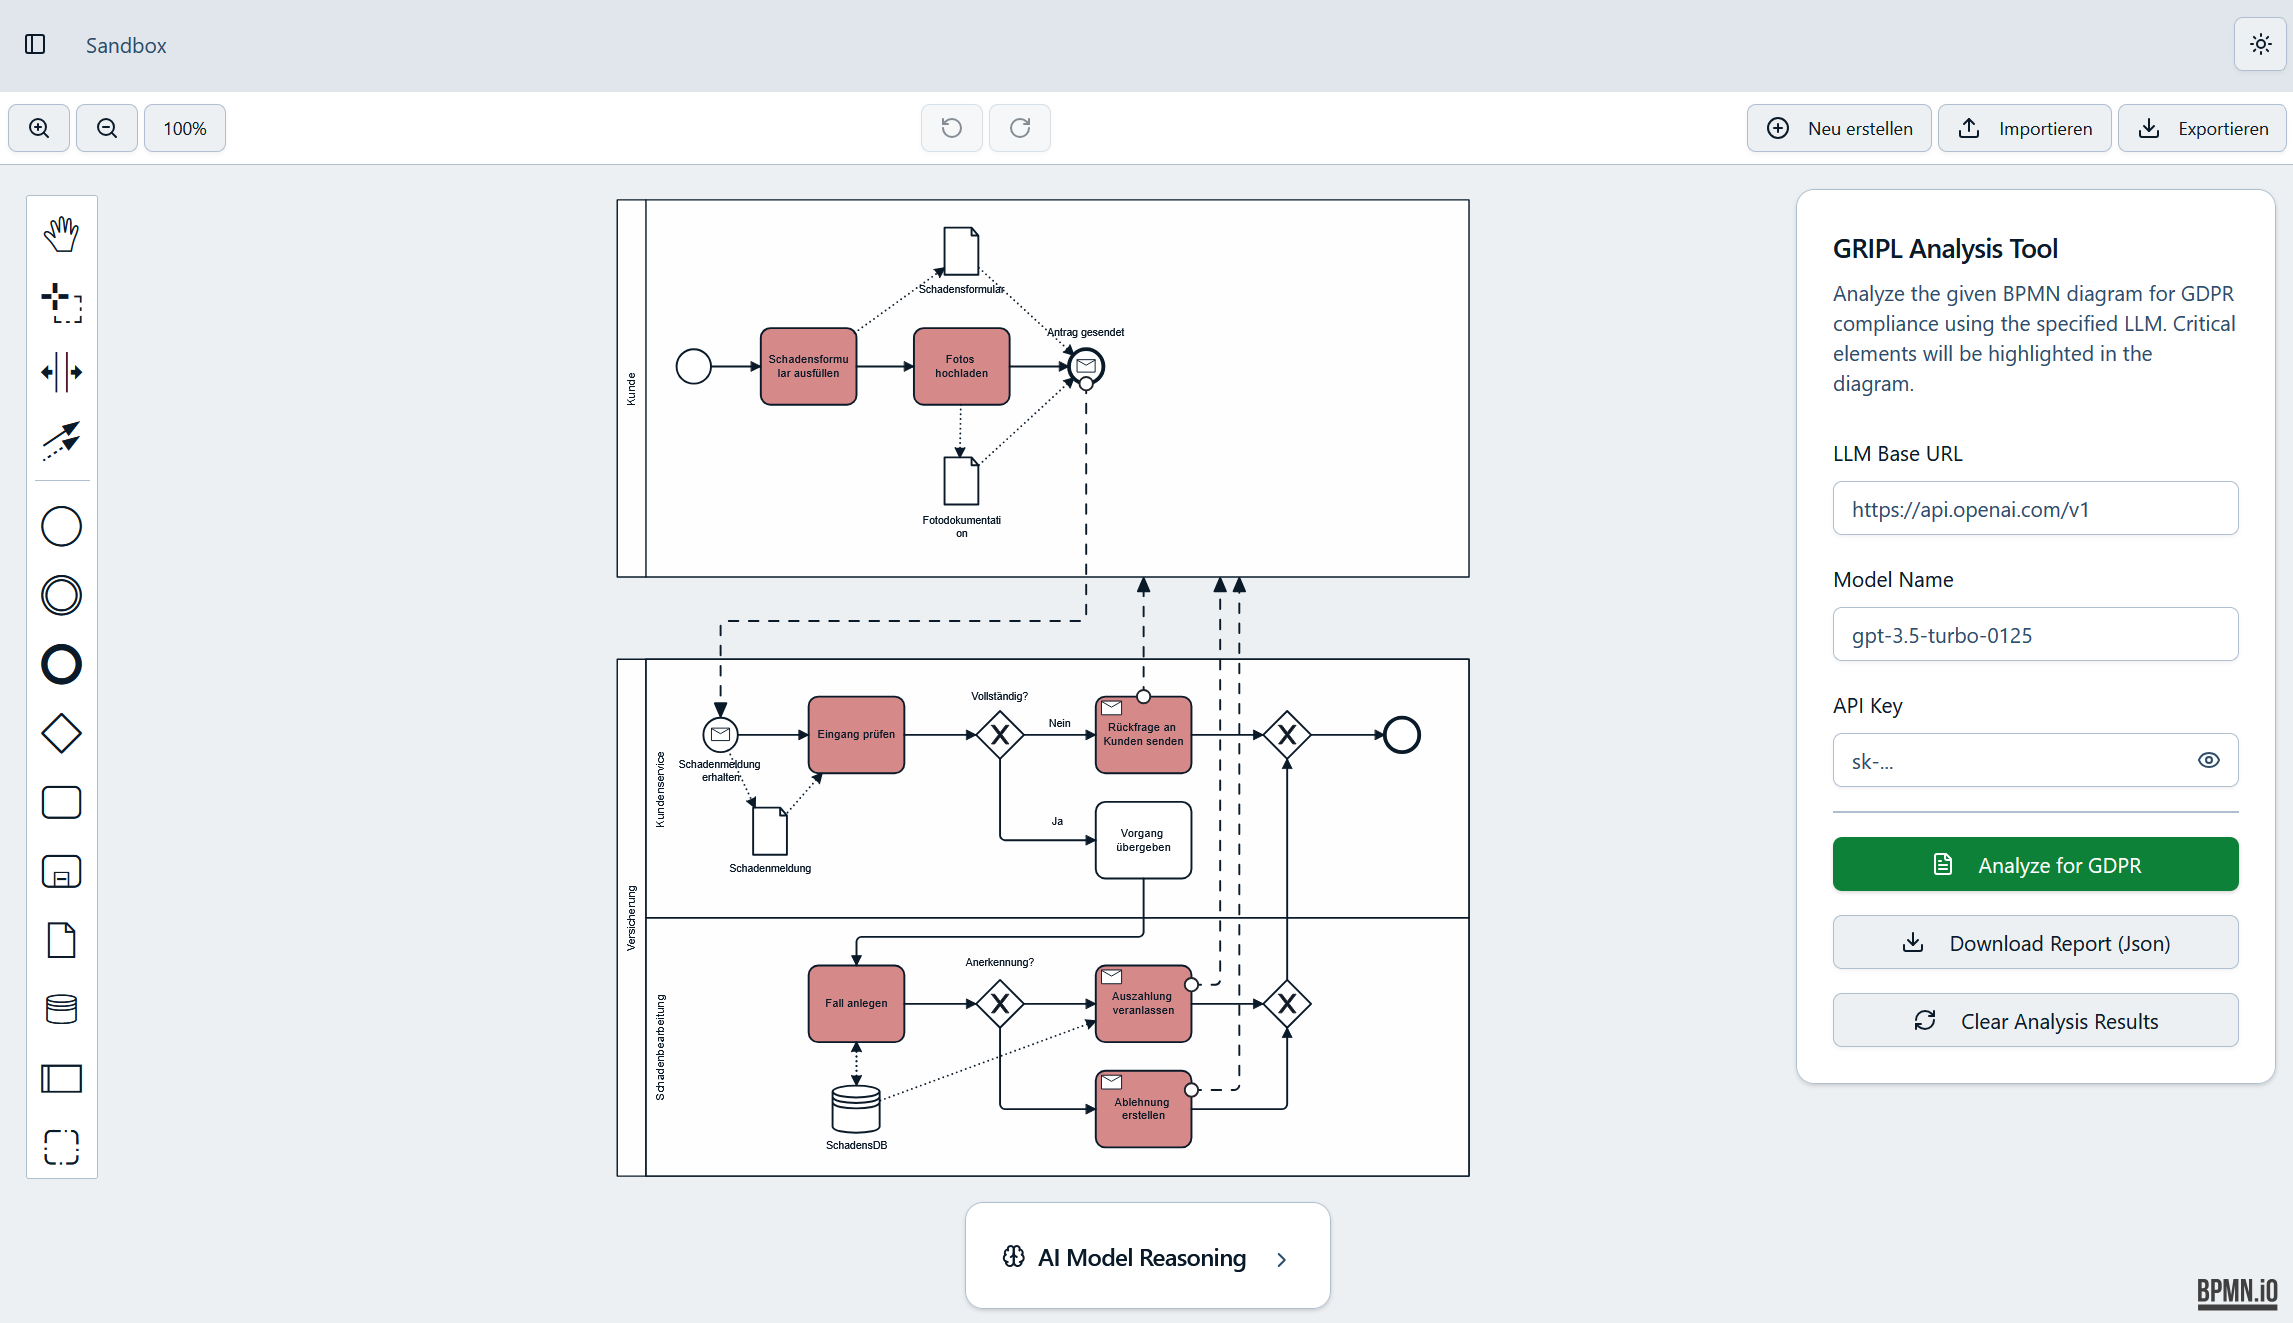
\includegraphics[width=\linewidth]{images/sandbox/sandbox-analyzed-model}
    \caption{Sandbox im Frontend mit hervorgehobenen kritischen Aktivitäten nach Analyse.}
    \label{fig:sandbox-frontend-analyzed-model}
\end{figure}

Außerdem können die vom \ac{LLM} generierten Begründungen zu jeder als kritisch erkannten Aktivität im Editor eingesehen werden. Diese Erläuterungen werden gesammelt in einer aufklappbaren Karte im unteren Bereich des Editors angezeigt, siehe Abbildung \ref{fig:sandbox-frontend-ai-reasoning}.

\begin{figure}
    \centering
    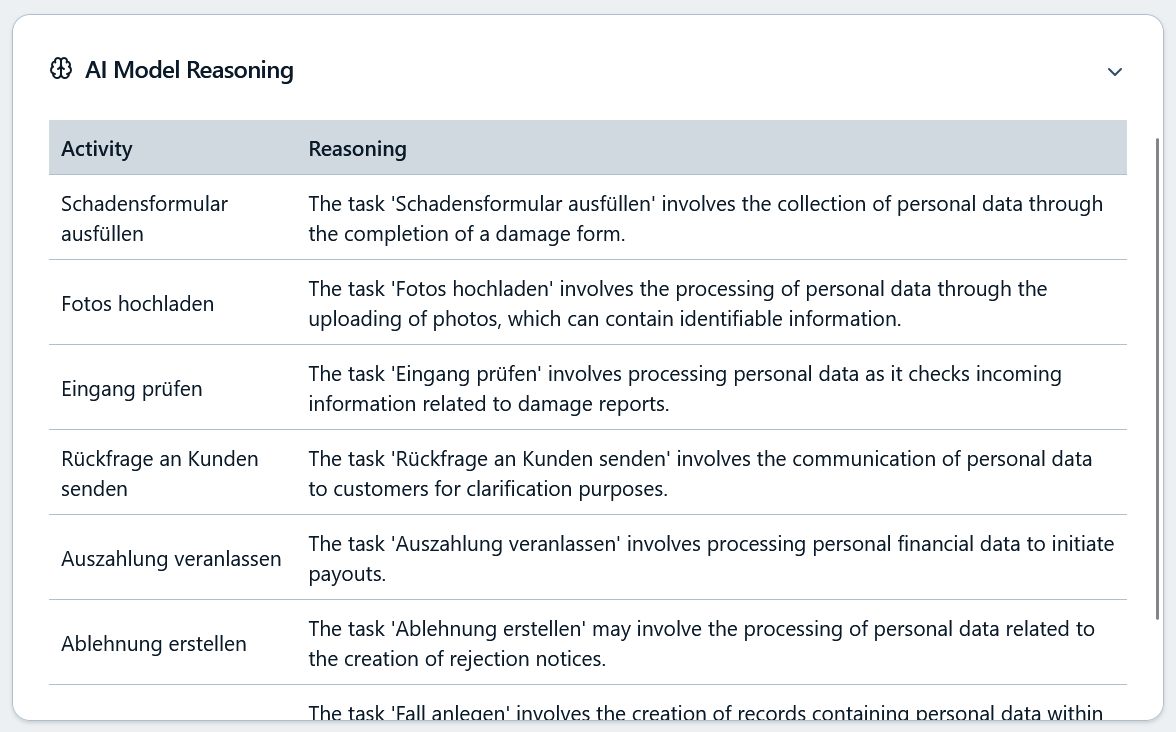
\includegraphics[width=\linewidth]{images/sandbox/sandbox-ai-reasoning}
    \caption{Begründung der Klassifikation durch das LLM in der Sandbox.}
    \label{fig:sandbox-frontend-ai-reasoning}
\end{figure}

Um verschiedene \acp{LLM} vergleichen zu können, verfügt die Sandbox auf der rechten Seite über ein Einstellungsmenü mit konfigurierbaren \ac{LLM}-Parametern (siehe Abbildung \ref{fig:sandbox-frontend-analyzed-model}). Diese Parameter sind identisch zu den in Kapitel \ref{sec:api-design} beschriebenen \texttt{llmProps} und werden beim Starten der Analyse in die API-Anfrage überführt.